\PassOptionsToPackage{table}{xcolor}
\documentclass[sigconf,review,anonymous]{acmart}
% ---------------------------------------------------------------------------------------------------------------
% Counting Sources, Not Pages -- WWW full paper.
% Every number in the text comes from ../results/ (summary.md, metrics.json); see paper/scripts/check_numbers.py.
% figures:  python paper/scripts/make_figures.py   (reads ../results/**.json and per-instance predictions)
% tables:   python paper/scripts/make_tables.py    (re-styles ../results/latex/*.tex, numbers copied verbatim)
% ---------------------------------------------------------------------------------------------------------------
\usepackage{booktabs}
\usepackage{tikz}
\usetikzlibrary{positioning,arrows.meta,fit,backgrounds,calc,shapes.misc}
\usepackage{enumitem}
\usepackage{pifont}

% ---- colours (shared with the figures) ----
\definecolor{oursred}{HTML}{C8102E}
\definecolor{voteblue}{HTML}{4A90C8}
\definecolor{hdrc}{gray}{0.86}
\definecolor{rowc}{gray}{0.955}
\definecolor{grpc}{HTML}{E4ECF5}
\definecolor{oursc}{HTML}{FCEBEE}
\definecolor{bestc}{HTML}{1F4E9A}
\definecolor{posc}{HTML}{1E7B34}
\definecolor{negc}{HTML}{C0392B}
\definecolor{nsigc}{gray}{0.55}
\definecolor{wrongc}{HTML}{F6D5D9}
\definecolor{rightc}{HTML}{D6E6F4}

% ---- table styling: gray/white banding, coloured header / group / our rows ----
\setlength{\aboverulesep}{0pt}
\setlength{\belowrulesep}{0pt}
\renewcommand{\arraystretch}{1.13}
\newcommand{\hdr}{\rowcolor{hdrc}}
\newcommand{\ours}{\rowcolor{oursc}}
\newcommand{\grp}[2]{\rowcolor{grpc}\multicolumn{#1}{l}{\footnotesize\bfseries\itshape #2}\\}
\newcommand{\best}[1]{\textbf{\textcolor{bestc}{#1}}}
\newcommand{\scnd}[1]{\underline{#1}}
\newcommand{\sigp}[1]{\textbf{\textcolor{posc}{#1}}}
\newcommand{\sign}[1]{\textbf{\textcolor{negc}{#1}}}
\newcommand{\nsig}[1]{\textcolor{nsigc}{#1}}

\newcommand{\sys}{\textsc{IndieRAG}}
\newcommand{\ess}{\mathrm{ESS}}
\newcommand{\pp}{\,pp}
\newcommand{\para}[1]{\smallskip\noindent\textbf{#1}\enspace}

\setlength{\emergencystretch}{1.5em}
\raggedbottom
\setcopyright{none}
\acmConference[WWW '27]{The ACM Web Conference 2027}{2027}{}
\acmYear{2027}
\settopmatter{printacmref=false}

\begin{document}
\title{Counting Sources, Not Pages: Dependence-Aware Evidence Aggregation against Illusory Consensus in Web RAG}

\author{Anonymous Author(s)}
\affiliation{\institution{Anonymous Institution}\country{}}

\begin{abstract}
Retrieval-augmented generation (RAG) over the Web treats every retrieved page as an independent witness, so a claim
repeated on many pages wins. Many of those pages share one origin: syndicated articles, scraped mirrors and
LLM-written content farms restate a single source in many surface forms. We call the result \emph{illusory consensus}
and show that it misleads current RAG systems. On EchoBench, a benchmark built from real web search results in which
one wrong origin and its copies compete with independent correct pages, eight copies drop the accuracy of a
Qwen2.5-7B reader from 86.5\% to 49.5\% and that of per-document majority voting to 24.5\%. Near-duplicate removal
and semantic deduplication recover little, because paraphrased, translated and summarised copies are not near
duplicates. We propose \sys{}, which brings copy detection from truth discovery to RAG. It estimates whether two
pages share an origin from lexical, semantic, rare-fact and machine-text signals, groups pages into origin clusters,
and weighs each claim by its effective number of independent sources. \sys{} raises echo accuracy by 17.3 and 11.0
points over vanilla RAG for two 8B-class readers (10.1 and 5.8 points over the strongest of 12 baselines), keeps
clean accuracy, and stays nearly flat as copies accumulate. Its shared-origin detector reaches 99.6 AUC, where
deduplication reaches 54 to 60, and costs 6\,ms per query on a CPU. On RAMDocs, \sys{} improves over vanilla RAG
by 6.2 and 10.4 points. On 6{,}397 real Bing result pages, 27.4\% of the pages share an origin with another page of
the same result list, 2.5 times the rate visible to near-duplicate detection.
\end{abstract}

\begin{CCSXML}
<ccs2012>
<concept><concept_id>10002951.10003317.10003347.10003348</concept_id>
<concept_desc>Information systems~Question answering</concept_desc><concept_significance>500</concept_significance></concept>
<concept><concept_id>10002951.10003260.10003277</concept_id>
<concept_desc>Information systems~Web mining</concept_desc><concept_significance>300</concept_significance></concept>
</ccs2012>
\end{CCSXML}
\ccsdesc[500]{Information systems~Question answering}
\ccsdesc[300]{Information systems~Web mining}
\keywords{retrieval-augmented generation, misinformation, copy detection, truth discovery, AI-generated content}

\maketitle

% =====================================================================================================================
\section{Introduction}
% =====================================================================================================================
Truth-discovery research showed for structured data that copying between sources breaks majority voting, and that
modelling the copying recovers the truth~\cite{dong2009integrating,li2015truthsurvey}. RAG systems built on Web search still count pages. A reader that
sees ten pages, seven of which give the same answer, takes the seven as corroboration, even when they are one article
syndicated seven times. Such duplication is now cheap. News is syndicated, Q\&A and trivia sites are scraped and
mirrored, LLMs rewrite one page into many fluent variants at almost no cost, and neural retrievers rank LLM-written
text above human-written text~\cite{dai2024neural}. Corpus-poisoning attacks exploit the same weakness by injecting
a handful of agreeing passages~\cite{zou2024poisonedrag}. A claim that appears on many pages but comes from one
origin produces \emph{illusory consensus} (Figure~\ref{fig:overview}a).

Existing defences judge passages one at a time or reward agreement between them. Work on knowledge conflicts studies
how readers weigh retrieved context against parametric
memory~\cite{xu2024conflicts,wu2024clasheval,ming2025faitheval,su2024conflictbank,chen2026ragknow}, and robust-RAG
methods filter, isolate or re-weight
passages~\cite{wang2024astute,wei2025instructrag,zhou2025trustrag,xiang2024robustrag,pan2024cag,deng2024cram,wang2025ramdocs}.
Reliability estimation by cross-source agreement~\cite{hwang2024rarag} even rewards copying, because copies always
agree. Near-duplicate removal~\cite{broder1997resemblance} and semantic deduplication~\cite{abbas2023semdedup} catch
verbatim mirrors, yet the copies that LLM rewriting produces are paraphrases, translations and summaries.

We treat the problem as copy detection over anonymous web text and make four contributions.
\begin{enumerate}[leftmargin=*,itemsep=1pt,topsep=2pt]
\item We define illusory consensus and build EchoBench from real TriviaQA search results. One wrong origin and up to
eight copies of five types, written by two LLMs or by rule, compete with independent correct pages. Control settings
separate repetition from LLM style and from independent disagreement.
\item We show that four readers from two model families, up to 32B parameters, lose 16 to 20 points of accuracy on
average under echoes and up to 37 points with eight copies. Majority voting over pages collapses, and deduplication
and robust-RAG baselines recover part of the loss.
\item We propose \sys{} (Figure~\ref{fig:overview}b), which estimates shared origin, clusters pages, and aggregates
claims by their effective sample size (ESS), either as a vote (IndieVote), as an evidence table for the reader, or as
a stopping signal for a search agent (IndieSearch). A copy-corrected Condorcet argument explains why page counting
fails and how detector recall governs the repair.
\item \sys{} improves echo accuracy by 17.3 and 11.0 points over vanilla RAG, significantly over all 12 baselines, with
unchanged clean accuracy. It also improves on RAMDocs, which has natural conflicts. On 1{,}000 real Bing result lists,
27.4\% of the pages share an origin with another retrieved page, against 10.9\% detectable as lexical near-duplicates.
\end{enumerate}

\begin{figure*}[t]
\centering
\makebox[\textwidth][c]{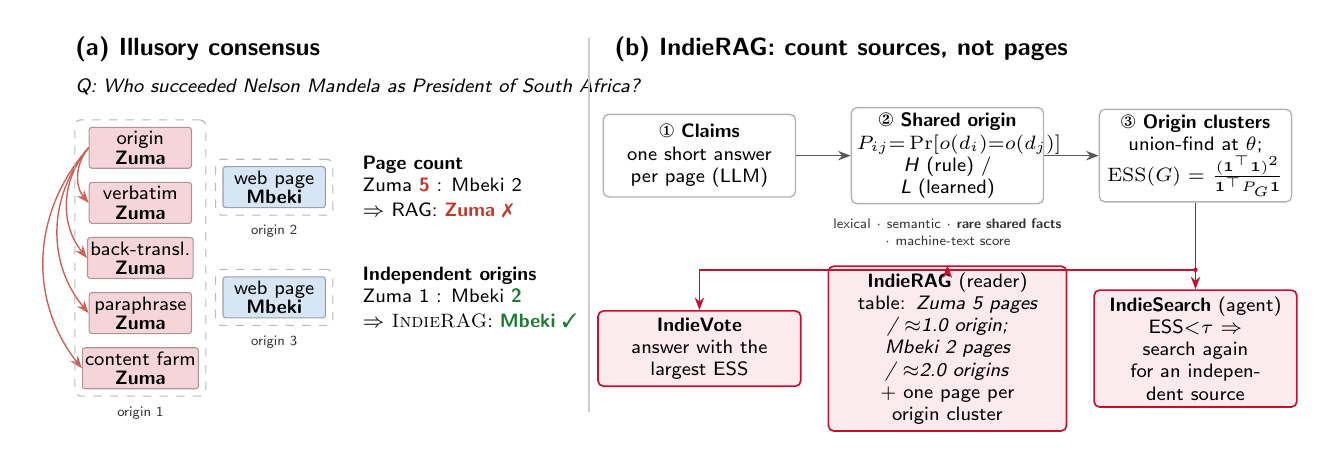
\begin{tikzpicture}[
  font=\sffamily\scriptsize, >={Stealth[length=1.6mm]},
  page/.style={draw=#1!70!black, fill=#1, rounded corners=1pt, minimum width=13mm, minimum height=5.2mm,
               align=center, inner sep=1pt, line width=0.4pt},
  stage/.style={draw=gray!60, fill=white, rounded corners=2pt, align=center, minimum height=10.5mm,
                text width=23mm, inner sep=2pt, line width=0.5pt},
  outbox/.style={draw=oursred, fill=oursc, rounded corners=2pt, align=center, text width=24mm, inner sep=2.5pt,
              line width=0.6pt},
  lbl/.style={font=\sffamily\tiny, text=gray!40!black}]
% ---------------- left: the problem ----------------
\node[font=\sffamily\small\bfseries, anchor=west] at (-0.2,2.5) {(a) Illusory consensus};
\node[anchor=west, font=\sffamily\scriptsize\itshape] at (-0.2,2.02)
  {Q: Who succeeded Nelson Mandela as President of South Africa?};
\node[page=wrongc] (o)  at (0.75,1.25) {origin\\[-1pt]\textbf{Zuma}};
\node[page=wrongc] (c1) at (0.75,0.55) {verbatim\\[-1pt]\textbf{Zuma}};
\node[page=wrongc] (c2) at (0.75,-0.15) {back-transl.\\[-1pt]\textbf{Zuma}};
\node[page=wrongc] (c3) at (0.75,-0.85) {paraphrase\\[-1pt]\textbf{Zuma}};
\node[page=wrongc] (c4) at (0.75,-1.55) {content farm\\[-1pt]\textbf{Zuma}};
\foreach \c in {c1,c2,c3,c4} {\draw[->, negc!80, line width=0.5pt] (o.west) to[bend right=40] (\c.west);}
\node[page=rightc] (g1) at (2.45,0.75) {web page\\[-1pt]\textbf{Mbeki}};
\node[page=rightc] (g2) at (2.45,-0.65) {web page\\[-1pt]\textbf{Mbeki}};
\node[draw=gray!55, dashed, rounded corners=2pt, fit=(o)(c4), inner sep=2.5pt, label={[lbl]below:origin 1}] {};
\node[draw=gray!55, dashed, rounded corners=2pt, fit=(g1), inner sep=2.5pt, label={[lbl]below:origin 2}] {};
\node[draw=gray!55, dashed, rounded corners=2pt, fit=(g2), inner sep=2.5pt, label={[lbl]below:origin 3}] {};
\node[align=left, anchor=west] at (3.45,0.75)
  {\textbf{Page count}\\ Zuma \textcolor{negc}{\textbf{5}} : Mbeki 2\\[1pt]
   $\Rightarrow$ RAG: \textcolor{negc}{\textbf{Zuma}} \textcolor{negc}{\ding{55}}};
\node[align=left, anchor=west] at (3.45,-0.65)
  {\textbf{Independent origins}\\ Zuma 1 : Mbeki \textcolor{posc}{\textbf{2}}\\[1pt]
   $\Rightarrow$ \sys{}: \textcolor{posc}{\textbf{Mbeki}} \textcolor{posc}{\ding{51}}};
\draw[gray!40, line width=0.6pt] (6.45,2.65) -- (6.45,-2.1);
% ---------------- right: the pipeline ----------------
\node[font=\sffamily\small\bfseries, anchor=west] at (6.65,2.5) {(b) \sys{}: count sources, not pages};
\node[stage] (s1) at (7.85,1.15) {\textbf{\ding{172} Claims}\\ one short answer\\ per page (LLM)};
\node[stage] (s2) at (11.0,1.15) {\textbf{\ding{173} Shared origin}\\ $P_{ij}{=}\Pr[o(d_i){=}o(d_j)]$\\ \textit{H} (rule) / \textit{L} (learned)};
\node[stage] (s3) at (14.15,1.15) {\textbf{\ding{174} Origin clusters}\\ union-find at $\theta$;\\ $\ess(G)=\frac{(\mathbf 1^\top \mathbf 1)^2}{\mathbf 1^\top P_G \mathbf 1}$};
\node[lbl, text width=30mm, align=center, below=0.6mm of s2]
  {lexical $\cdot$ semantic $\cdot$ \textbf{rare shared facts}\\ $\cdot$ machine-text score};
\draw[->, gray!70!black, line width=0.6pt] (s1) -- (s2);
\draw[->, gray!70!black, line width=0.6pt] (s2) -- (s3);
\node[outbox] (v)  at (7.85,-1.3) {\textbf{IndieVote}\\ answer with the\\ largest ESS};
\node[outbox, text width=28.5mm] (r)  at (11.0,-1.3) {\textbf{\sys{}} (reader)\\ table: \emph{Zuma 5 pages / ${\approx}$1.0 origin;\\ Mbeki 2 pages / ${\approx}$2.0 origins}\\ + one page per origin cluster};
\node[outbox] (a)  at (14.15,-1.3) {\textbf{IndieSearch} (agent)\\ ESS${<}\tau$ $\Rightarrow$ search again\\ for an independent source};
\draw[oursred, line width=0.6pt] (s3.south) -- (14.15,-0.3);
\draw[oursred, line width=0.6pt] (7.85,-0.3) -- (14.15,-0.3);
\foreach \t/\x in {v/7.85,r/11.0,a/14.15} {\draw[->, oursred, line width=0.6pt] (\x,-0.3) -- (\t.north);}
\fill[oursred] (14.15,-0.3) circle (0.8pt);
\end{tikzpicture}
}
\vspace{-1mm}
\caption{\textbf{Overview.} (a) Illusory consensus in a schematic example: one wrong origin echoed by four copies
out-counts two independent correct pages. (b) \sys{} estimates which pages share an origin and aggregates claims by
their effective number of independent sources (ESS), as a vote, as an evidence table with one page per origin for the
reader, or as a stopping signal for a search agent.}
\label{fig:overview}
\end{figure*}

% =====================================================================================================================
\section{Related Work}
% =====================================================================================================================
\para{Truth discovery and copy detection.} Dong et al.~\cite{dong2009integrating} showed that copying between
structured sources misleads voting and estimated truth, source accuracy and copying jointly (ACCU and its copy-aware
extensions); Li et al.~\cite{li2015truthsurvey} survey the area. Sharing \emph{rare or false} values is strong
evidence of copying, an observation that motivates our rare-fact signal. We move the idea from structured claims of
named sources to anonymous web pages, where both claims and dependence must be inferred from free text and where LLM
rewriting hides copying from string matching.

\para{Knowledge conflicts and robust RAG.} Surveys and benchmarks study conflicts between context and
memory~\cite{xu2024conflicts,wu2024clasheval,ming2025faitheval,su2024conflictbank,chen2026ragknow}. RAMDocs and
MADAM-RAG~\cite{wang2025ramdocs} combine ambiguity, misinformation and noise and resolve them by multi-agent debate.
Astute RAG~\cite{wang2024astute} consolidates internal and external knowledge, InstructRAG~\cite{wei2025instructrag}
generates rationales, TrustRAG~\cite{zhou2025trustrag} filters suspicious clusters, RobustRAG~\cite{xiang2024robustrag}
isolates passages and aggregates their answers, and CAG and CrAM~\cite{pan2024cag,deng2024cram} condition generation on
credibility. RA-RAG~\cite{hwang2024rarag} estimates source reliability by cross-checking sources. Self-RAG and
CRAG~\cite{asai2023selfrag,yan2024crag} decide when to retrieve or correct. PoisonedRAG~\cite{zou2024poisonedrag}
injects several adversarial passages per target question, which is illusory consensus created on purpose.

\para{Deduplication and machine-text detection.} Shingling with containment and resemblance, approximated at scale by
MinHash and LSH~\cite{broder1997resemblance}, SimHash fingerprints for web crawling~\cite{manku2007nearduplicates}, and
embedding-based SemDeDup~\cite{abbas2023semdedup} remove near-identical documents with a binary similarity decision. Paraphrased or summarised copies fall below such
thresholds, and independent pages about the same fact can exceed them. Zero-shot detectors such as
Fast-DetectGPT~\cite{bao2024fastdetectgpt} and Binoculars~\cite{hans2024binoculars} flag LLM text; we use such a score
as one weak feature.

\para{Search agents.} Search-R1~\cite{jin2025searchr1} and R1-Searcher~\cite{song2025r1searcher} train agents with RL to
interleave search and reasoning~\cite{lin2025agenticsearch}. These agents stop once retrieved evidence agrees, and
echoes make agreement cheap.

% =====================================================================================================================
\section{Problem and a Copy-Corrected Condorcet View}\label{sec:theory}
% =====================================================================================================================
A question $q$ comes with retrieved pages $D=\{d_1,\dots,d_n\}$. Each page supports at most one candidate answer
$a(d_i)$ and is generated by an unobserved \emph{origin} $o(d_i)$; pages with the same origin are verbatim, translated,
paraphrased, summarised or rewritten copies of each other. A group $G_a=\{d: a(d)=a\}$ shows \emph{illusory consensus}
when $|G_a|$ is large and the number of distinct origins $|\{o(d):d\in G_a\}|$ is small. Page-level aggregation,
explicit (majority vote) or implicit (a reader swayed by repetition), estimates $|G_a|$. The quantity that carries
evidence is the number of origins.

\begin{proposition}[Copy-corrected Condorcet]\label{prop}
Let $n$ origins be independently correct with probability $p>\frac12$ in a binary decision, and let one origin be
copied $m$ times. Let $A_m$ be the accuracy of majority voting over pages, with ties broken uniformly. Then $A_0$ is
the Condorcet accuracy $\Pr[\mathrm{Bin}(n,p)>\frac n2]$ plus half the tie mass, and $A_m=p$ for every $m\geq n-1$:
the copied origin alone decides the vote. If each copy is detected and merged into its origin independently with
probability $r$, the accuracy is $\mathbb{E}[A_U]$ with $U\sim\mathrm{Bin}(m,1-r)$ undetected copies. It equals $A_0$
for $r=1$ and decays to $p$ as $m(1-r)$ grows.
\end{proposition}
\begin{proof}[Proof sketch]
The copied origin contributes $m{+}1$ identical votes and the other $n{-}1$ origins at most $n{-}1$ votes. For $m+1>n-1$
the copied origin is always in the majority, so the vote is correct exactly when that origin is, with probability $p$.
Merging detected copies leaves $U$ extra votes, and conditioning on $U$ gives the mixture.
\end{proof}
A simulation with $n{=}5$, $p{=}0.65$ and $2\cdot10^5$ trials confirms this (Figure~\ref{fig:theory}a). Page voting
falls from 76.3\% to 64.9 to 65.1\% once $m\geq4$, while a perfect detector stays at 76.3 to 76.6\% for all $m\leq32$.
With recall $0.8$ the accuracy at $m{=}32$ is 65.4\%, so a detector has to catch nearly every copy, paraphrases
included, to help against heavy echoing.

\begin{figure}[!t]
\centering
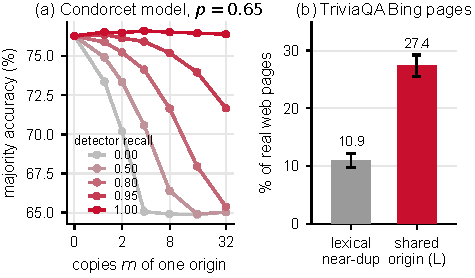
\includegraphics[width=\linewidth]{figures/theory_web.pdf}
\vspace{-5mm}
\caption{(a) Simulation of Proposition~\ref{prop}: majority accuracy over pages vs.\ copies of one origin, for
detectors of increasing recall. (b) Real web pages (TriviaQA Bing results, 6{,}397 pages) that have a lexical
near-duplicate vs.\ that share an origin with another page of the same result list according to \sys{}-L
(95\% bootstrap CIs).}
\label{fig:theory}
\vspace{-2mm}
\end{figure}

% =====================================================================================================================
\section{EchoBench}\label{sec:bench}
% =====================================================================================================================
\para{Source data.} We sample 1{,}000 of the 6{,}376 TriviaQA rc.web~\cite{joshi2017triviaqa} validation questions whose
cached Bing results contain at least four pages from distinct domains that mention the gold answer. Up to three of
these real pages, truncated to 220 words, serve as \emph{independent correct} evidence.

\para{Wrong origin and copies.} A builder LLM (Qwen2.5-7B-Instruct) proposes a plausible wrong answer (valid for 984
questions) and rewrites another real page of the question so that it states this answer (a valid \emph{origin} for
760 questions). From the origin we produce eight copies of each of five types: \emph{verbatim} syndication (rule-based,
with random site boilerplate and optional truncation), \emph{back-translation} through one of five pivot languages,
\emph{paraphrase}, \emph{content-farm} rewriting with one of four personas, and \emph{summary}. Half of the paraphrase
and content-farm copies come from a second generator, Phi-3.5-mini-instruct, which lets us test transfer across
generators. A copy is kept only if it still states the wrong answer and does not mention the gold answer; the filter
keeps 99.2\% of the verbatim copies and 73 to 85\% of the LLM-written ones, 25{,}142 copies in total. For each question
we also write three \emph{independent wrong} pages from different base pages without showing the origin, and sample 12
distractor pages from other questions. The 760 questions are split by question into 304 training questions, used only
to train the dependence classifier and to select demonstrations, and 456 test questions.

\para{Settings.} \textbf{A (main):} one wrong origin with $m\in\{0,1,2,4,8\}$ mixed-type copies against
$k\in\{1,2,3\}$ independent correct pages and two distractors, shuffled. For $k\geq2$ the independent majority is
correct for every $m$; for $k{=}1$ the origins are tied and the reader's own knowledge decides.
\textbf{Types:} $m{=}4$ copies of a single type, $k{=}2$. \textbf{B:} $m\in\{1,2,3\}$ \emph{independent} wrong pages
without copies against $k{=}2$; a method should follow the independent majority here, and B-agree measures whether it
does. \textbf{Style:} the correct pages are LLM-paraphrased as well, so that machine-written text no longer signals a
wrong answer. \textbf{C:} the true page with $m\in\{2,4\}$ copies against $w\in\{1,2\}$ independent wrong pages.
\textbf{Ranked:} pages in dense-retriever (bge-base) order. \textbf{Noisy:} $d\in\{0,6,10\}$ additional distractors.
Real pages keep their true domains. Generated pages receive a domain from a list of fictitious sites and a simulated
date, with copies dated after their origin; the metadata variant L+meta therefore serves only as a reference point.

\para{HotpotQA-echo and RAMDocs.} For search agents we build 300 HotpotQA~\cite{yang2018hotpotqa} distractor-dev
questions in which the answer-bearing gold paragraph is rewritten into a wrong origin with four copies, added to a local
search index of 14{,}236 passages. RAMDocs~\cite{wang2025ramdocs} (500 questions) provides natural conflicts from
ambiguity, misinformation and noise, with an imbalanced number of supporting documents and no synthetic copies.

% =====================================================================================================================
\section{Method: IndieRAG}\label{sec:method}
% =====================================================================================================================
\para{Claims.} The reader extracts one short answer per page with the instruction ``answer only from this document, or
NONE''. Answers are grouped by normalised string equality, containment or token-F1${\geq}0.6$. All claim-based methods
(majority vote, ACCU, IndieVote, IndieBayes and \sys{}) share this step.

\para{Shared-origin estimation.} For every pair of pages we estimate $P_{ij}=\Pr[o(d_i)=o(d_j)]$ from four cheap feature
groups.
(i)~\emph{Lexical}: 5-gram and 3-gram Jaccard and 5-gram containment.
(ii)~\emph{Semantic}: bge-base cosine and its gap to 3-gram overlap, which is large for paraphrases.
(iii)~\emph{Rare shared facts}: independent sources share common facts but seldom the same rare
details~\cite{dong2009integrating}. From each page we extract numbers, capitalised phrases and words with IDF$\geq4$
(excluding question terms) and use the IDF-weighted overlap of the shared set, its maximum IDF and its size.
(iv)~\emph{Machine text}: the minimum and maximum over the pair of a Fast-DetectGPT~\cite{bao2024fastdetectgpt}
curvature score (Qwen2.5-1.5B), plus the length ratio.
\textbf{H} is a training-free rule,
$P_{ij}=\max\!\big(c_5,\ \sigma(12(\rho_{ij}-0.3))\cdot\mathbb{1}[\cos_{ij}>0.7]\big)$, with $c_5$ the 5-gram
containment and $\rho_{ij}$ the rare-fact overlap. \textbf{L} is a gradient-boosted classifier (300 trees) trained on
238{,}581 page pairs from the 304 training questions only. \textbf{LLM} asks the reader whether two passages derive from
the same source, for candidate pairs with cosine${\geq}0.75$ or 3-gram Jaccard${\geq}0.1$.

\para{Origin clusters and effective sample size.} Pages are clustered by union-find over edges $P_{ij}\geq\theta$
($\theta{=}0.5$). For an answer group $G$ with weights $w$ (uniform here), the effective number of independent sources is
the Kish effective sample size under correlation $P$:
\begin{equation}
\ess(G)=\frac{\left(\sum_{i\in G}w_i\right)^2}{w_G^{\top}P_G\,w_G},\qquad P_G=[P_{ij}]_{i,j\in G},\ P_{ii}=1.
\end{equation}
It equals $|G|$ for independent pages and 1 for $|G|$ exact copies, and changes smoothly with uncertain $P$.

\para{Aggregators.} \textbf{IndieVote} returns the answer with the largest ESS, breaking ties by page count.
\textbf{IndieBayes} is a copy-aware ACCU-style update~\cite{dong2009integrating}: supporting pages are ordered by
estimated accuracy and the vote of $d_i$ is discounted by $\prod_{j\prec i}(1-0.9P_{ij})$ over 5 EM iterations.
\textbf{\sys{}} gives the reader an \emph{evidence table} that lists, for each candidate answer, the number of pages
and the approximate number of independent origins, sorted by ESS, together with one representative page (the longest)
per origin cluster. The prompt asks the reader to weigh independent origins and to use its own knowledge when the
evidence is balanced, which resolves the tied case $k{=}1$ that a vote cannot.

\para{IndieSearch.} A ReAct-style agent~\cite{jin2025searchr1} receives, after every search, an
\texttt{<evidence\_status>} block with the pages and ESS of each candidate answer. If it tries to answer while the
leading answer has $\ess<\tau$ ($\tau{=}1.5$), it is asked once to search again with a differently phrased query that
excludes pages already seen and pages with cosine${>}0.9$ to them.

\begin{table*}[t]
\centering
\caption{\textbf{Illusory consensus on EchoBench (setting A).} Accuracy (\%) without copies (Clean), with $m{=}8$
copies of one wrong origin against $k{=}2$ independent correct pages, and averaged over all $m\!\geq\!1$, $k\!\in\!\{1,2,3\}$
(Echo, 12 conditions $\times$ 200 test questions). Wrong$\downarrow$: rate of outputting the injected wrong answer
(Echo conditions). Slope: $d\,\mathrm{acc}/d\log_2(m{+}1)$ at $k{=}2$ (0 = flat). B-agr.: agreement with the
independent majority in control setting B ($m{=}1$ or $3$ independent wrong pages vs.\ $k{=}2$; no copies). Tok: reader tokens per instance (Qwen2.5-7B).
\best{Best} and \scnd{second best} exclude oracle rows and L+meta (simulated page metadata); ``--'': method run on a reduced condition set.}
\label{tab:main}
\setlength{\tabcolsep}{3.6pt}
\small
\rowcolors{3}{white}{rowc}
\begin{tabular}{l rrrrrr rrrrrr r}
\toprule
\hdr & \multicolumn{6}{c}{\textbf{Reader: Qwen2.5-7B-Instruct}} & \multicolumn{6}{c}{\textbf{Reader: Qwen3-8B}} & \\
\cmidrule(lr){2-7}\cmidrule(lr){8-13}
\hdr \textbf{Method} & Clean & $m{=}8$ & Echo & Wrong$\downarrow$ & Slope & B-agr. & Clean & $m{=}8$ & Echo & Wrong$\downarrow$ & Slope & B-agr. & Tok \\
\midrule
\grp{14}{Single-pass readers}
Vanilla RAG & 80.7 & 49.5 & 61.0 & 31.9 & $-$0.119 & 55.9 & 85.2 & 59.5 & 68.5 & 26.7 & $-$0.090 & 59.0 & 2.5k \\
Near-dup removal & 80.8 & 53.5 & 64.0 & 28.5 & $-$0.106 & 55.6 & \scnd{85.3} & 58.0 & 70.4 & 24.7 & $-$0.094 & 59.0 & 2.3k \\
SemDeDup & 80.5 & 59.0 & 66.2 & 25.7 & $-$0.088 & 55.9 & 85.2 & 65.0 & 73.0 & 22.2 & $-$0.069 & 59.0 & 2.2k \\
TrustRAG (filter) & 80.5 & 51.0 & 62.2 & 30.1 & $-$0.114 & 55.6 & 85.2 & 61.5 & 70.1 & 25.0 & $-$0.083 & 58.7 & 2.5k \\
Astute RAG & 76.5 & 61.0 & 67.4 & 13.3 & $-$0.050 & 45.0 & 70.2 & 26.0 & 46.3 & \best{7.9} & $-$0.137 & 38.9 & 2.8k \\
InstructRAG-ICL & \best{87.3} & 58.0 & 66.8 & 31.7 & $-$0.102 & 63.3 & \best{87.3} & 69.0 & 73.6 & 34.8 & $-$0.067 & 64.6 & 2.7k \\
CAG (prompted) & \scnd{86.8} & 57.5 & 68.1 & 29.4 & $-$0.099 & 65.1 & 84.7 & 68.5 & 73.7 & 22.6 & $-$0.064 & 56.6 & 5.3k \\
\grp{14}{Per-document claims + aggregation}
Majority vote & 75.7 & 24.5 & 35.0 & 57.2 & $-$0.203 & 67.9 & 78.2 & 27.5 & 40.6 & 51.6 & $-$0.200 & \best{68.4} & 3.0k \\
Near-dup + vote & 75.7 & 29.0 & 42.7 & 49.9 & $-$0.190 & 67.9 & 78.2 & 31.5 & 47.7 & 45.0 & $-$0.189 & \best{68.4} & 3.0k \\
SemDeDup + vote & 75.7 & 33.5 & 46.8 & 45.9 & $-$0.171 & 67.9 & 78.2 & 36.5 & 51.3 & 41.4 & $-$0.170 & \best{68.4} & 3.0k \\
ACCU (no copy det.) & 75.7 & 24.5 & 35.0 & 57.2 & $-$0.203 & 67.9 & 78.2 & 27.5 & 40.6 & 51.6 & $-$0.200 & \best{68.4} & 3.0k \\
MADAM-RAG & -- & 54.0 & -- & -- & -- & -- & -- & 46.5 & -- & -- & -- & -- & 11.9k \\
\grp{14}{Ours: dependence-aware vote}
\ours IndieVote-H & 75.8 & 75.5 & 63.1 & 30.6 & $-$0.032 & \best{70.5} & 78.2 & \scnd{79.0} & 67.1 & 25.8 & \scnd{$-$0.027} & \best{68.4} & 3.0k \\
\ours IndieVote-L & 75.8 & 76.0 & 63.6 & 30.6 & $-$0.030 & \best{70.5} & 78.0 & \scnd{79.0} & 67.1 & 26.0 & \scnd{$-$0.027} & \scnd{67.5} & 3.0k \\
\ours IndieVote-LLM & 75.7 & 65.0 & 59.2 & 34.7 & $-$0.066 & \scnd{68.8} & 78.0 & 71.0 & 63.2 & 29.8 & $-$0.054 & 65.8 & 10.0k \\
\ours IndieBayes-L & 75.8 & 75.5 & 63.1 & 30.9 & $-$0.032 & \best{70.5} & 78.0 & 78.5 & 66.9 & 26.1 & $-$0.029 & \scnd{67.5} & 3.0k \\
\grp{14}{Ours: dependence-aware reader}
\ours \sys-H & 81.3 & \scnd{78.0} & \scnd{77.5} & \best{12.9} & $-$0.028 & 62.7 & 83.7 & 78.0 & \scnd{78.8} & \scnd{14.0} & \best{$-$0.025} & 59.8 & 4.6k \\
\ours \sys-L & 80.3 & \best{80.0} & \best{78.3} & \scnd{13.2} & \best{$-$0.017} & 63.3 & 84.7 & \best{79.5} & \best{79.5} & 14.3 & \scnd{$-$0.027} & 62.1 & 4.9k \\
\ours \sys-L+meta & 81.3 & 84.0 & 79.7 & 11.9 & $-$0.007 & 61.9 & 84.5 & 82.5 & 81.4 & 12.5 & $-$0.018 & 61.4 & 4.7k \\
\ours \sys-LLM & 82.8 & \scnd{78.0} & \scnd{77.5} & 14.0 & \scnd{$-$0.025} & 62.2 & 83.8 & \best{79.5} & 78.5 & 15.0 & \best{$-$0.025} & 58.1 & 12.0k \\
\grp{14}{Oracle dependence (upper bound)}
IndieVote-oracle & 75.7 & 76.5 & 63.6 & 30.4 & $-$0.029 & 67.9 & 78.2 & 80.5 & 67.5 & 25.7 & $-$0.023 & 68.4 & 3.0k \\
\sys-oracle & 82.2 & 85.5 & 81.4 & 9.9 & $-$0.002 & 64.4 & 84.7 & 85.5 & 83.8 & 10.8 & $-$0.010 & 63.3 & 4.7k \\
\bottomrule
\end{tabular}
\end{table*}

% =====================================================================================================================
\section{Experimental Setup}\label{sec:setup}
% =====================================================================================================================
\para{Readers.} Qwen2.5-7B-Instruct (primary) and Qwen3-8B run on the full grid; Granite-3.3-8B-Instruct (second family)
and Qwen2.5-32B-Instruct-AWQ (scale) run settings A and B with six methods. All use vLLM, greedy decoding and an 8k
context.

\para{Baselines.} Vanilla RAG. \emph{Deduplication before reading:} 5-gram containment${\geq}0.5$, the quantity
MinHash/LSH approximates~\cite{broder1997resemblance}, and SemDeDup~\cite{abbas2023semdedup} (bge cosine${\geq}0.95$).
\emph{Claims and aggregation:} majority vote (isolate-then-aggregate as in RobustRAG~\cite{xiang2024robustrag}), the
same vote after near-duplicate or SemDeDup clustering (``Near-dup + vote'' and ``SemDeDup + vote'', which are IndieVote
with a binary similarity-based dependence), and ACCU without copy detection (source-accuracy truth
discovery~\cite{dong2009integrating}, the within-query analogue of RA-RAG~\cite{hwang2024rarag}).
\emph{Robust RAG:} Astute RAG~\cite{wang2024astute}, InstructRAG-ICL~\cite{wei2025instructrag}, TrustRAG's filtering
stage~\cite{zhou2025trustrag}, MADAM-RAG~\cite{wang2025ramdocs} with one agent per document and two debate rounds, and
CAG in prompted form~\cite{pan2024cag}, where the reader rates each page's credibility from 1 to 10 and sees the
ratings. All baselines use the same reader; variants that need fine-tuning (InstructRAG-FT, CAG and CrAM training,
cross-query RA-RAG) are outside our scope.

\para{Budget.} Each reader is evaluated on the first 200 test questions, 6{,}537 instances for the full grid.
Expensive methods run on subsets of condition groups, and every average covers only conditions that all compared
methods ran on (``--'' otherwise); MADAM-RAG, for example, ran at $m\in\{0,2,8\}$, $k{=}2$.

\para{Metrics and statistics.} \emph{Accuracy}: the output contains a gold alias. \emph{Wrong}: it contains the
injected wrong answer. On RAMDocs, accuracy requires all valid answers and no misinformation answer. Paired
differences use a question-clustered bootstrap with 5{,}000 resamples, since instances of one question are dependent,
and Holm correction over the 12 baselines. An LLM judge (Qwen3-8B) re-grading 700 EchoBench predictions agrees with
string matching on 97.4\% of them (Cohen $\kappa{=}0.94$, ranking Kendall $\tau{=}0.80$). On RAMDocs agreement is
81.4\% ($\kappa{=}0.56$), mostly because string matching misses paraphrased multi-answers, and the method ranking is
preserved ($\tau{=}0.92$; Table~\ref{tab:judge}).

% =====================================================================================================================
\section{Results}\label{sec:results}
% =====================================================================================================================

\subsection{Echoes mislead RAG readers}\label{sec:rq1}
\para{Accuracy falls with every added copy.} With $k{=}2$ independent correct pages, Qwen2.5-7B's accuracy falls from
86.5\% at $m{=}0$ to 71.0\%, 61.5\% and 49.5\% at $m{=}2,4,8$ (Figure~\ref{fig:susc}b). Three independent correct pages
still lose ground to one origin echoed eight times (87.5\% to 52.5\%, Figure~\ref{fig:susc}c). Qwen3-8B follows the
same curve (88.0\% to 59.5\% at $k{=}2$), and so does the 32B reader, which drops from 88.0\% clean to 63.0\% at
$m{=}8$ (Table~\ref{tab:readers}). The wrong outputs are the echoed answer: 31.9\% of all echo-condition outputs
contain it (Table~\ref{tab:main}).

\begin{figure*}[t]
\centering
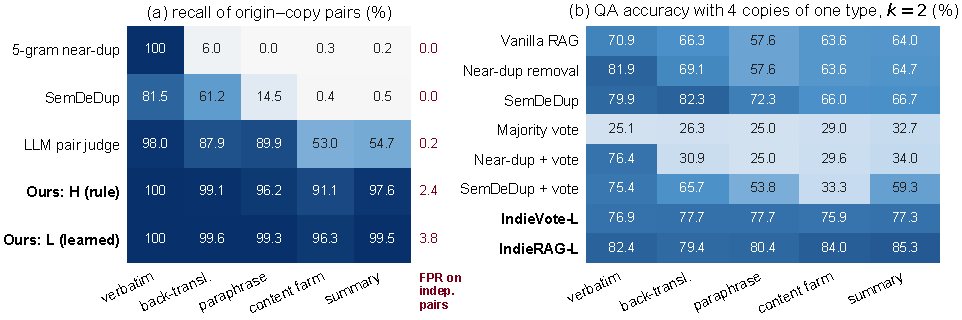
\includegraphics[width=\textwidth]{figures/copytypes.pdf}
\vspace{-5mm}
\caption{\textbf{By copy type.} (a) Recall of origin--copy pairs at threshold 0.5 per estimator, and false-positive rate on
independent pairs (right column). (b) Accuracy with four copies of a single type ($k{=}2$, Qwen2.5-7B; 150 to 199
questions per type). Lexical and embedding deduplication miss paraphrase, content-farm and summary copies, which the
learned estimator finds.}
\label{fig:copytypes}
\vspace{-1mm}
\end{figure*}
\para{Voting over pages amplifies the problem.} Per-document majority vote, the literal form of page counting,
collapses to 24.5\% at $m{=}8$ with a slope of $-$0.203, against $-$0.119 for vanilla RAG. ACCU-style truth discovery
without copy detection is identical to it in every condition, because copies agree with each other and so appear
reliable.

\begin{figure*}[t]
\centering
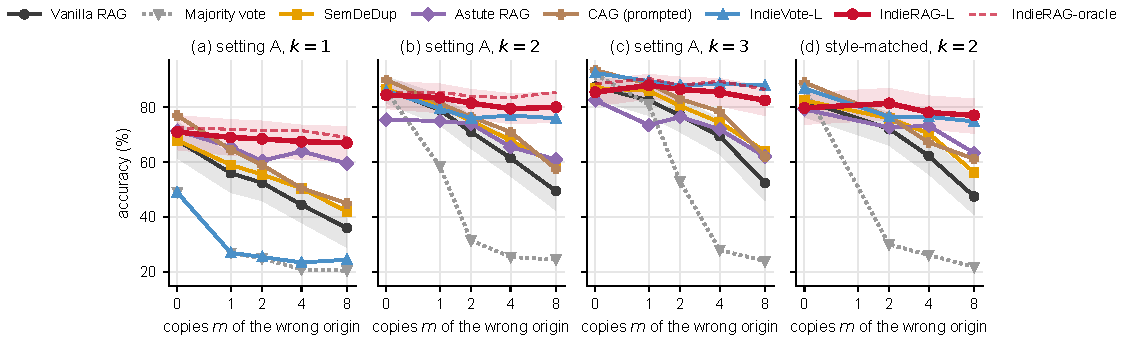
\includegraphics[width=\textwidth]{figures/susceptibility.pdf}
\vspace{-5mm}
\caption{\textbf{Accuracy vs.\ number of copies of one wrong origin} (Qwen2.5-7B). (a to c) Setting A with $k$
independent correct pages, 200 test questions per point; (d) style-matched control in which the correct pages are
LLM-rewritten as well, 183 questions per point. Shaded: 95\% bootstrap bands for vanilla RAG and \sys{}-L. Majority
vote (dotted) collapses; \sys{}-L (red) stays nearly flat and close to the oracle-dependence upper bound (dashed).}
\label{fig:susc}
\vspace{-1mm}
\end{figure*}

\para{Deduplication removes only verbatim echoes.} Near-duplicate removal raises accuracy with verbatim copies from
70.9\% to 81.9\% and leaves paraphrases (57.6\%) and content-farm rewrites (63.6\%) at the vanilla level
(Figure~\ref{fig:copytypes}b). SemDeDup also catches back-translations (82.3\%) and misses content-farm copies (66.0\%)
and summaries (66.7\%). Over all echo conditions, the two raise accuracy from 61.0\% to 64.0\% and 66.2\%.

\para{Robust-RAG baselines help partially and depend on the reader.} Astute RAG answers conservatively, with the lowest
wrong-answer rate among baselines (13.3\%), and reaches 67.4\% echo accuracy with Qwen2.5-7B, 46.3\% with Qwen3-8B and
27.1\% with Granite. InstructRAG-ICL and prompted CAG have the best clean accuracy (87.3\% and 86.8\%) and still slope
down ($-$0.102 and $-$0.099). MADAM-RAG reaches 54.0\% at $m{=}8$ with 4.8 times the tokens of vanilla RAG.

\subsection{Counting sources restores accuracy}\label{sec:rq2}
\para{Main result.} \sys{}-L reaches 78.3\% echo accuracy with Qwen2.5-7B and 79.5\% with Qwen3-8B, against
61.0\% and 68.5\% for vanilla RAG and 68.1\% and 73.7\% for the strongest baseline, prompted CAG. The paired gains are
+17.3\pp{} [13.4, 21.0] and +11.0\pp{} [7.5, 14.7] over vanilla RAG and +10.1\pp{} [6.5, 13.7] and +5.8\pp{}
[2.5, 9.1] over CAG, and all 24 comparisons with the 12 baselines are significant after Holm correction
(Table~\ref{tab:sig}). The slope flattens from $-$0.119 to $-$0.017, the wrong-answer rate falls from 31.9\% to
13.2\%, and clean accuracy is unchanged (80.3\% vs.\ 80.7\%; 84.7\% vs.\ 85.2\%). The training-free estimator H
reaches 77.5\% and 78.8\%, so most of the gain is available without training data, and oracle origins reach 81.4\% and
83.8\%.

\begin{table}[!t]
\centering
\caption{\textbf{Paired gains of \sys{}-L over each baseline} ($\Delta$acc in points). EchoBench: setting A, $m\!\geq\!1$
(2{,}400 instances; 400 for MADAM-RAG); RAMDocs: 500 questions. Question-clustered bootstrap, Holm-corrected over the
12 baselines: $^{\ddagger}p_{\text{Holm}}{<}0.01$, $^{\dagger}p_{\text{Holm}}{<}0.05$; \sigp{green}/\sign{red} =
significant gain/loss, \nsig{gray} = not significant. CIs in Appendix~\ref{app:tables}.}
\label{tab:sig}
\setlength{\tabcolsep}{4pt}
\small
\rowcolors{3}{white}{rowc}
\begin{tabular}{l rr rr}
\toprule
\hdr & \multicolumn{2}{c}{\textbf{EchoBench}} & \multicolumn{2}{c}{\textbf{RAMDocs}} \\
\cmidrule(lr){2-3}\cmidrule(lr){4-5}
\hdr \textbf{vs.\ baseline} & Qwen2.5 & Qwen3 & Qwen2.5 & Qwen3 \\
\midrule
Vanilla RAG & \sigp{+17.3}$\,^{\ddagger}$ & \sigp{+11.0}$\,^{\ddagger}$ & \sigp{+6.2}$\,^{\dagger}$ & \sigp{+10.4}$\,^{\ddagger}$ \\
Near-dup removal & \sigp{+14.3}$\,^{\ddagger}$ & \sigp{+9.1}$\,^{\ddagger}$ & \nsig{$-$3.4} & \nsig{$-$1.4} \\
SemDeDup & \sigp{+12.0}$\,^{\ddagger}$ & \sigp{+6.5}$\,^{\ddagger}$ & \nsig{+2.8} & \sigp{+6.6}$\,^{\dagger}$ \\
Majority vote & \sigp{+43.3}$\,^{\ddagger}$ & \sigp{+38.9}$\,^{\ddagger}$ & \nsig{+0.6} & \sigp{+10.0}$\,^{\ddagger}$ \\
Near-dup + vote & \sigp{+35.6}$\,^{\ddagger}$ & \sigp{+31.8}$\,^{\ddagger}$ & \nsig{$-$0.2} & \sigp{+9.2}$\,^{\ddagger}$ \\
SemDeDup + vote & \sigp{+31.5}$\,^{\ddagger}$ & \sigp{+28.2}$\,^{\ddagger}$ & \nsig{+0.6} & \sigp{+10.0}$\,^{\ddagger}$ \\
Astute RAG & \sigp{+10.8}$\,^{\ddagger}$ & \sigp{+33.2}$\,^{\ddagger}$ & \nsig{+4.6} & \sigp{+28.6}$\,^{\ddagger}$ \\
InstructRAG-ICL & \sigp{+11.4}$\,^{\ddagger}$ & \sigp{+5.9}$\,^{\ddagger}$ & \nsig{+5.2} & \nsig{+4.0} \\
TrustRAG (filter) & \sigp{+16.1}$\,^{\ddagger}$ & \sigp{+9.4}$\,^{\ddagger}$ & \sigp{+5.8}$\,^{\dagger}$ & \sigp{+10.8}$\,^{\ddagger}$ \\
MADAM-RAG & \sigp{+17.8}$\,^{\ddagger}$ & \sigp{+26.8}$\,^{\ddagger}$ & \sigp{+6.8}$\,^{\dagger}$ & \sigp{+20.2}$\,^{\ddagger}$ \\
CAG (prompted) & \sigp{+10.1}$\,^{\ddagger}$ & \sigp{+5.8}$\,^{\ddagger}$ & \sigp{+7.8}$\,^{\dagger}$ & \sigp{+7.0}$\,^{\ddagger}$ \\
ACCU (no copy det.) & \sigp{+43.3}$\,^{\ddagger}$ & \sigp{+38.9}$\,^{\ddagger}$ & \sigp{+6.8}$\,^{\dagger}$ & \sigp{+16.2}$\,^{\ddagger}$ \\
\bottomrule
\end{tabular}
\end{table}


\para{The vote and the reader complement each other.} IndieVote-L turns the collapsing majority vote into a flat curve
(76.0\% at $m{=}8$, $k{=}2$, against 24.5\%) and follows the independent majority in setting B more often than majority
vote does (B-agree 70.5\% vs.\ 67.9\%), so genuine agreement between independent pages still counts. With $k{=}1$
the wrong origin and the correct page are one origin each, and the vote falls back to page counts (24.5\% at $m{=}8$),
which lowers its echo average to 63.6\%. \sys{} hands this tie to the reader's knowledge and keeps 67.0\% at $k{=}1$,
$m{=}8$, against 36.0\% for vanilla RAG.

\begin{table}[!t]
\centering
\caption{\textbf{Controls and stress tests} (Qwen2.5-7B, accuracy \% unless noted).
\emph{Style}: correct pages also LLM-rewritten ($m{=}8$). \emph{Rank.}: documents in dense-retriever order ($m{=}8$).
\emph{Noise}: 10 distractor pages ($m{=}4$). \emph{B-agr.}: follows the independent majority when wrong sources are
independent. \emph{Setting C}: copies of the \emph{true} page vs.\ $w$ independent wrong pages; C-ind.: agreement
with the independent majority at $m{=}4$, $w{=}2$. Questions per condition: style 183, ranked and noise 200, setting C
93, 98 and 68. Shaded: ours.}
\label{tab:controls}
\setlength{\tabcolsep}{1.6pt}
\small
\rowcolors{3}{white}{rowc}
\begin{tabular}{l rrrr rrr}
\toprule
\hdr & \multicolumn{4}{c}{\textbf{Echoed misinformation}} & \multicolumn{3}{c}{\textbf{Setting C (echoed truth)}} \\
\cmidrule(lr){2-5}\cmidrule(lr){6-8}
\hdr \textbf{Method} & Style & Rank. & Noise & B-agr. & {\scriptsize $m4,w1$} & {\scriptsize $m2,w2$} & C-ind. \\
\midrule
Vanilla RAG & 47.5 & 56.5 & 57.0 & 55.9 & 87.1 & 78.6 & 10.3 \\
SemDeDup & 56.3 & -- & 65.5 & 55.9 & -- & -- & -- \\
Majority vote & 21.9 & 24.0 & 26.0 & \scnd{67.9} & \best{93.5} & \best{85.7} & 5.9 \\
SemDeDup + vote & 31.1 & 33.5 & 40.5 & \scnd{67.9} & \best{93.5} & 79.6 & 5.9 \\
Astute RAG & 63.4 & 54.5 & -- & 45.0 & 84.9 & \best{85.7} & 5.9 \\
CAG (prompted) & 61.2 & -- & -- & 65.1 & \scnd{92.5} & \scnd{84.7} & 10.3 \\
\ours IndieVote-L & \scnd{74.9} & \scnd{76.5} & \scnd{76.5} & \best{70.5} & \best{93.5} & 44.9 & \best{45.6} \\
\ours IndieBayes-L & 73.8 & \scnd{76.5} & 75.5 & \best{70.5} & \best{93.5} & 44.9 & \scnd{44.1} \\
\ours \sys-L & \best{77.0} & \best{79.0} & \best{81.0} & 63.3 & 75.3 & 64.3 & 27.9 \\
\bottomrule
\end{tabular}
\end{table}


\para{Controls for style, order and noise.} All wrong pages in EchoBench are LLM-written, so a method could learn that
machine-written text is wrong. When the correct pages are LLM-rewritten as well, \sys{}-L keeps
77.0\% at $m{=}8$ against 47.5\% for vanilla RAG (Table~\ref{tab:controls}, Figure~\ref{fig:susc}d), and dropping the
machine-text feature changes IndieVote-L's echo accuracy by 0.0 and +0.1 points (Table~\ref{tab:ablation}).
Retriever-ordered pages (79.0\% vs.\ 56.5\% at $m{=}8$) and ten extra distractors (81.0\% vs.\ 57.0\%) give the same
picture. Setting C shows what the method optimises. When the true page is the echoed one and two independent pages
disagree with it, the independent majority is wrong; IndieVote follows the independent majority as designed (44.9\%
accuracy at $m{=}2$, $w{=}2$), page counting follows the echo (85.7\%), and \sys{}-L, whose reader can override a
balanced table, lies in between (64.3\%).

\begin{table}[!t]
\centering
\caption{\textbf{Ablations} (accuracy \%). Echo columns: \sign{red}/\sigp{green} = at least 1 point below/above the
first row of the block. ms: dependence estimation per instance (CPU). $^{*}$Page metadata in EchoBench is simulated
(see \S\ref{sec:bench}), so L+meta is optimistic.}
\label{tab:ablation}
\setlength{\tabcolsep}{2.6pt}
\small
\rowcolors{3}{white}{rowc}
\begin{tabular}{l rrr r rr}
\toprule
\hdr & \multicolumn{3}{c}{\textbf{Qwen2.5-7B}} & \textbf{Qwen3} & & \\
\cmidrule(lr){2-4}\cmidrule(lr){5-5}
\hdr \textbf{Variant} & Clean & Echo & B-agr. & Echo & ms & Tok \\
\midrule
\grp{7}{Reader input (\sys{}-L)}
\sys{}-L (full) & \textbf{80.3} & \textbf{78.3} & \textbf{63.3} & \textbf{79.5} & \textbf{6} & \textbf{4.9k} \\
\quad table + all docs & 82.3 & \sign{62.5} & 61.5 & \sign{67.3} & 6 & 5.3k \\
\quad grouped docs, no table & 78.8 & 79.2 & 62.1 & 80.4 & 6 & 4.6k \\
\grp{7}{Dependence estimator (\sys{})}
\quad H (rule) & \textbf{81.3} & \textbf{77.5} & \textbf{62.7} & \textbf{78.8} & \textbf{3} & \textbf{4.6k} \\
\quad LLM pair judge & 82.8 & 77.5 & 62.2 & 78.5 & 121 & 12.0k \\
\quad L + page metadata$^{*}$ & 81.3 & \sigp{79.7} & 61.9 & \sigp{81.4} & 5 & 4.7k \\
\quad oracle origins & 82.2 & \sigp{81.4} & 64.4 & \sigp{83.8} & 0 & 4.7k \\
\grp{7}{Feature groups (IndieVote-L)}
IndieVote-L (all features) & \textbf{75.8} & \textbf{63.6} & \textbf{70.5} & \textbf{67.1} & \textbf{6} & \textbf{3.0k} \\
\quad $-$lexical & 75.8 & 63.5 & 70.5 & 67.2 & 6 & 3.0k \\
\quad $-$semantic & 75.8 & 63.4 & 70.5 & 67.2 & 6 & 3.0k \\
\quad $-$rare facts & 75.8 & 62.9 & 69.6 & 66.3 & 6 & 3.0k \\
\quad $-$machine-text score & 75.8 & 63.6 & 69.6 & 67.2 & 6 & 3.0k \\
\quad lexical only & 75.7 & \sign{61.6} & 69.6 & \sign{65.8} & 6 & 3.0k \\
\bottomrule
\end{tabular}
\end{table}


\para{Grouping pages by origin is the main mechanism.} Table~\ref{tab:ablation} varies the reader input. With the
evidence table but all pages in context, echo accuracy is 62.5\%: the reader is still swayed by the copies it reads.
Showing one page per origin cluster gives 79.2\% even without the table. The table adds 1.5 points of clean accuracy and
helps on RAMDocs (32.2\% vs.\ 27.8\% and 41.0\% vs.\ 36.2\%, Table~\ref{tab:ramdocs}). Among the features, the rare-fact group matters most end to end (63.6\% to 62.9\% and 67.1\%
to 66.3\% without it), and a lexical-only classifier loses 2.0 and 1.3 points. The clustering threshold matters
little: at $m{=}8$, $k{=}2$, $\theta\in\{0.3,0.5,0.7\}$ gives 77.5, 80.0 and 81.5\%.

\subsection{Across readers and on natural conflicts}\label{sec:readers}
\begin{figure}[!t]
\centering
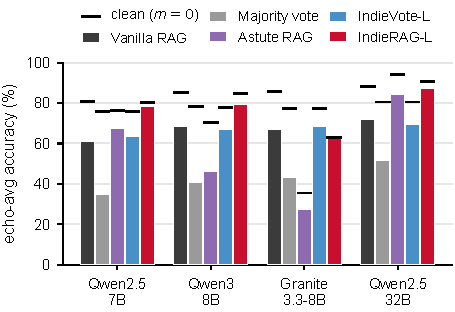
\includegraphics[width=\linewidth]{figures/readers.pdf}
\vspace{-5mm}
\caption{Echo accuracy (bars) and clean accuracy (black ticks) across reader families and scales. IndieVote-L needs no
reader prompt and beats majority vote for every reader; \sys{}-L gives the largest gains for readers that use its
evidence table.}
\label{fig:readers}
\vspace{-2mm}
\end{figure}
Figure~\ref{fig:readers} summarises the four readers. At 32B, \sys{}-L reaches 87.3\% echo accuracy against 72.1\% for
vanilla RAG and 84.4\% for Astute RAG, the strongest baseline there. The vote and the reader variant suit different
readers: Granite-3.3-8B makes poor use of the grouped prompt (63.2\% clean accuracy with it, 85.8\% without), and for
this reader the prompt-free IndieVote-L is the better choice (68.6\% vs.\ 67.0\% for vanilla RAG). On RAMDocs, with
natural conflicts and no synthetic copies, \sys{}-L improves over vanilla RAG by +6.2\pp{} (Holm $p{=}0.020$) and
+10.4\pp{} ($p{=}0.002$) and over MADAM-RAG, the method proposed with RAMDocs, by +6.8 and +20.2 points; 5-gram
deduplication performs on par here (35.6\% and 42.4\%, differences n.s.; Table~\ref{tab:ramdocs}), which suggests
that RAMDocs' imbalanced support comes mostly from near-identical documents.


\subsection{Shared origin is detectable}\label{sec:rq3}
On the 456 test pools, L reaches 99.6 AUC (95\% CI [99.5, 99.7]) and an origin-clustering ARI of 0.882
(Table~\ref{tab:dep}). The deduplication estimators reach 53.8 and 60.0 AUC: they find verbatim copies (100\% and
81.5\% recall) and almost none of the content-farm copies or summaries (at most 0.5\%, Figure~\ref{fig:copytypes}a).
The LLM pair judge is precise (0.2\% false positives), recalls 53.0\% of content-farm and 54.7\% of summary copies, and
takes 5.4\,s per pool against 24\,ms for L on a CPU. Rare shared facts carry the most information (ARI 0.882 to 0.799
without them), and 25 training questions already give 99.5 AUC. The hardest negatives are independent pages that state
the \emph{same} wrong answer as the copies (8.9\% false positives) or the same correct answer (4.9\%).

\begin{table}[!t]
\centering
\caption{\textbf{Shared-origin detection} on the pools of the 456 EchoBench test questions (189{,}746 pairs, 59.5\%
dependent). AUC/AP/F1@0.5 in \%; ARI of the origin clustering at $\theta{=}0.5$; ms per pool. $^{*}$Simulated metadata.}
\label{tab:dep}
\setlength{\tabcolsep}{3.5pt}
\small
\rowcolors{3}{white}{rowc}
\begin{tabular}{l rrrrr}
\toprule
\hdr \textbf{Estimator} & AUC & AP & F1 & ARI & ms \\
\midrule
\grp{6}{Estimators}
5-gram near-dup ($\geq$0.5) & 53.8 & 62.5 & 14.2 & 0.096 & 1 \\
SemDeDup (cos $\geq$0.95) & 60.0 & 67.6 & 33.4 & 0.320 & 0 \\
LLM pair judge (Qwen2.5-7B) & 95.0 & 94.5 & 76.2 & \best{0.923} & 5388 \\
\ours Ours: H (rule, no training) & \scnd{99.2} & \scnd{99.4} & \scnd{96.9} & \scnd{0.904} & 26 \\
\ours Ours: L (learned) & \best{99.6} & \best{99.7} & \best{97.7} & 0.882 & 24 \\
\ours Ours: L + metadata$^{*}$ & 99.9 & 99.9 & 99.0 & 0.949 & 24 \\
\grp{6}{Ablations and learning curve of L}
\quad L $-$lexical & 99.6 & 99.7 & 97.7 & 0.880 & 24 \\
\quad L $-$semantic & 99.6 & 99.7 & 97.6 & 0.872 & 24 \\
\quad L $-$rare facts & 99.1 & 99.3 & 96.4 & 0.799 & 24 \\
\quad L $-$machine-text score & 99.6 & 99.7 & 97.8 & 0.881 & 24 \\
\quad L lexical only & 97.9 & 98.5 & 94.4 & 0.763 & 24 \\
\quad L, 25 training questions & 99.5 & 99.6 & 96.9 & 0.907 & 24 \\
\quad L, 100 training questions & 99.5 & 99.6 & 97.4 & 0.882 & 24 \\
\bottomrule
\end{tabular}
\end{table}

\para{Transfer.} Trained without any Phi-3.5 copies, L still recalls 94.2\% of that generator's content-farm copies and
93.3\% of its paraphrases (98.2\% and 97.9\% when trained on them). Applied unchanged to HotpotQA-echo, whose Wikipedia
paragraphs differ in style from web pages, L keeps 97.8 AUC with an AP of 73.6. The ESS computed from L is off by 0.12
origins on average, against 3.0 for page counts. In our pools the dense retriever ranks copies and correct pages
similarly (mean normalised ranks 0.42 to 0.55 vs.\ 0.425), and because copies are numerous, 85.5\% of top-3 lists
contain at least one LLM-written copy.

\subsection{Illusory consensus on real search results}\label{sec:web}
We apply L, trained only on EchoBench, to the unmodified cached Bing results of 1{,}000 further TriviaQA questions
(6{,}397 pages, 6.4 per question). 27.4\% [25.6, 29.2] of the pages fall into a dependent cluster, against 10.9\%
[9.7, 12.2] with a lexical near-duplicate (Figure~\ref{fig:theory}b), and the gold answer is supported by 1.45 times
as many pages as independent origins. These are model estimates, since real pages carry no origin labels. In this 2017
snapshot the dependence seldom changes the winning answer: of the 297 questions whose pages support two or more
answers, page and origin majorities disagree in 3.7\%.

\begin{table}[!t]
\centering
\caption{\textbf{Natural data: unmodified web search results} (TriviaQA, cached Bing pages; 1{,}000 questions, 297 of
them with pages supporting $\geq$2 answers = ``conf.''). Accuracy (\%) on all questions and paired difference to
vanilla RAG ($\Delta$, points) on all and on conflict questions (vanilla: 84.2/84.3\%).
\sigp{Green}/\sign{red}: 95\% CI above/below 0; \nsig{gray}: CI contains 0.}
\label{tab:web}
\setlength{\tabcolsep}{3pt}
\small
\rowcolors{4}{white}{rowc}
\begin{tabular}{l rrr rrr}
\toprule
\hdr & \multicolumn{3}{c}{\textbf{Qwen2.5-7B}} & \multicolumn{3}{c}{\textbf{Qwen3-8B}} \\
\cmidrule(lr){2-4}\cmidrule(lr){5-7}
\hdr \textbf{Method} & Acc & $\Delta$ & $\Delta$conf. & Acc & $\Delta$ & $\Delta$conf. \\
\midrule
Vanilla RAG & 91.3 & -- & -- & 92.1 & -- & -- \\
Near-dup removal & 90.8 & \sign{$-$0.5} & \sign{$-$1.3} & 91.8 & \nsig{$-$0.3} & \nsig{$-$0.4} \\
SemDeDup & 91.1 & \nsig{$-$0.2} & \nsig{$-$0.7} & 91.9 & \nsig{$-$0.2} & \nsig{+0.0} \\
Majority vote & 91.0 & \nsig{$-$0.3} & \nsig{$-$2.7} & 91.4 & \nsig{$-$0.7} & \nsig{$-$0.4} \\
SemDeDup + vote & 90.9 & \nsig{$-$0.4} & \nsig{$-$3.0} & 91.5 & \nsig{$-$0.6} & \nsig{+0.0} \\
Astute RAG & 80.0 & \sign{$-$11.3} & \sign{$-$11.4} & 68.9 & \sign{$-$23.2} & \sign{$-$22.8} \\
InstructRAG-ICL & 89.9 & \nsig{$-$1.4} & \nsig{+0.3} & 92.8 & \nsig{+0.7} & \sigp{+5.0} \\
TrustRAG (filter) & 90.9 & \sign{$-$0.4} & \nsig{$-$0.7} & 91.9 & \nsig{$-$0.2} & \nsig{+0.0} \\
CAG (prompted) & 91.9 & \nsig{+0.6} & \nsig{+2.0} & 91.4 & \nsig{$-$0.7} & \nsig{+1.4} \\
\ours IndieVote-L & 91.1 & \nsig{$-$0.2} & \nsig{$-$2.4} & 91.3 & \nsig{$-$0.8} & \nsig{$-$0.7} \\
\ours IndieBayes-L & 91.1 & \nsig{$-$0.2} & \nsig{$-$2.4} & 91.4 & \nsig{$-$0.7} & \nsig{$-$0.4} \\
\ours \sys-L & 89.2 & \sign{$-$2.1} & \nsig{$-$1.3} & 89.7 & \sign{$-$2.4} & \nsig{+1.4} \\
\bottomrule
\end{tabular}
\end{table}


On these pages IndieVote-L matches vanilla RAG (91.1\% vs.\ 91.3\% and 91.3\% vs.\ 92.1\%, both n.s.;
Table~\ref{tab:web}). \sys{}-L trades 2.1 and 2.4 points on all questions for its robustness to echoes, and on the
conflict questions its difference to vanilla RAG is not significant ($-$1.3 and +1.4\pp). We therefore recommend the
reader variant where echoed misinformation is expected, for example in poisoning-prone corpora, and IndieVote-L where
echoes are rare.

\subsection{Search agents and cost}\label{sec:agents}
With four copies in the index, IndieSearch answers 77.7\% of EchoBench questions correctly against 73.3\% for ReAct with
the same 7B policy and 67.7\% for the RL-trained Search-R1, and gives the echoed answer less often (14.7\% vs.\ 16.7\%
and 23.0\%; Table~\ref{tab:agents}). The paired gain over ReAct is +4.3\pp{} [$-$0.3, +9.3] ($p{=}0.080$, 300
questions). The seek-again rule carries the gain: evidence-status feedback alone ($\tau{=}0$) reaches 69.0\%. On
multi-hop HotpotQA-echo, prompted agents perform alike and Search-R1, trained on HotpotQA, is best.
\sys{}-L costs 9.5 LLM calls per instance (8.5 claim extractions with 17 generated tokens in total, plus one reader
call), 4.9k prompt tokens and two sequential rounds; dependence estimation takes 6\,ms on a CPU (Table~\ref{tab:cost},
Figure~\ref{fig:cost}). This is twice the tokens of vanilla RAG, similar to prompted CAG (5.2k), and less than half of
MADAM-RAG (11.2k tokens, 18.9 calls).

% =====================================================================================================================
\section{Scope and Ethics}\label{sec:limits}
% =====================================================================================================================
EchoBench copies come from two 4B to 7B LLMs and from rules, and copy validity is checked automatically (wrong answer
kept, gold answer absent); larger content-farm models may rewrite more freely, which the cross-generator test and the
natural-data results address in part. \sys{} measures independent support, so it follows independent majorities and
discounts echoed truths by design (settings B and C). The RAG readers were evaluated on 200 test questions each, and
the natural-data study uses a reproducible 2017 snapshot that predates LLM content farms. Shared-origin signals could
help adversaries diversify poisoned copies; the same signals make cheap mass rewriting less effective. We will
release the benchmark and code for defensive research. All source pages come from the public TriviaQA release.

% =====================================================================================================================
\section{Conclusion}
% =====================================================================================================================
RAG readers, robust-RAG methods and deduplication all treat echoes of one origin as corroboration. \sys{} estimates
shared origin from text and aggregates claims by their effective number of independent sources. On EchoBench this keeps
accuracy nearly flat as copies accumulate, with clean accuracy unchanged, and the detector finds the paraphrased and
content-farm copies that deduplication misses in milliseconds per query. On real Bing results it places more than a
quarter of the pages in an origin cluster with another retrieved page.

\bibliographystyle{ACM-Reference-Format}
\bibliography{refs}

% =====================================================================================================================
\appendix
\section{Additional Results}\label{app:tables}
% =====================================================================================================================
This appendix gives the search-agent results, the full significance tests with confidence intervals, the LLM-judge
validation, results per copy type and per reader, the cost breakdown, the controls for the second reader, RAMDocs, the
natural-data comparison with confidence intervals, and the accuracy-cost plot.

\begin{table}[!t]
\centering
\caption{\textbf{Search agents} (300 questions each, local dense search engine). $m$: copies of a wrong origin
injected into the index. \#S: searches per question.}
\label{tab:agents}
\setlength{\tabcolsep}{2.8pt}
\small
\rowcolors{3}{white}{rowc}
\begin{tabular}{l rrrr rrr}
\toprule
\hdr & \multicolumn{4}{c}{\textbf{EchoBench}} & \multicolumn{3}{c}{\textbf{HotpotQA-echo}} \\
\cmidrule(lr){2-5}\cmidrule(lr){6-8}
\hdr \textbf{Agent} & $m{=}0$ & $m{=}4$ & Wr.$\downarrow$ & \#S & $m{=}0$ & $m{=}4$ & \#S \\
\midrule
ReAct (Qwen2.5-7B) & 84.0 & 73.3 & \scnd{16.7} & 0.77 & 40.3 & 25.3 & 1.33 \\
Search-R1 (RL, 7B) & \best{87.3} & 67.7 & 23.0 & 1.57 & \best{47.0} & \best{32.0} & 2.42 \\
\ours IndieSearch ($\tau{=}1.5$) & \best{87.3} & \best{77.7} & \best{14.7} & 2.04 & \scnd{41.3} & 26.7 & 3.29 \\
\ours \quad feedback only ($\tau{=}0$) & \scnd{86.3} & 69.0 & 20.7 & 1.30 & \scnd{41.3} & 24.0 & 2.37 \\
\ours \quad stricter ($\tau{=}2$) & \scnd{86.3} & \scnd{73.7} & 18.3 & 2.55 & \scnd{41.3} & \scnd{27.0} & 3.34 \\
\bottomrule
\end{tabular}
\end{table}

\begin{table}[h]
\centering
\caption{Paired significance of \sys{}-L vs.\ every baseline: $\Delta$acc, 95\% question-clustered bootstrap CI,
bootstrap $p$, Holm-corrected $p$, and McNemar $p$ (reference).}
\label{tab:sigfull}
\setlength{\tabcolsep}{3pt}
\scriptsize
\rowcolors{2}{white}{rowc}
\begin{tabular}{l r r c r r r}
\toprule
\hdr \textbf{vs.\ baseline} & $n$ & $\Delta$acc & 95\% CI & $p$ & $p_{\text{Holm}}$ & $p_{\text{McN}}$ \\
\midrule
\grp{7}{EchoBench, Qwen2.5-7B}
Vanilla RAG & 2400 & +17.3 & [+13.4, +21.0] & <0.001 & 0.002 & <0.001 \\
Near-dup removal & 2400 & +14.3 & [+10.6, +18.0] & <0.001 & 0.002 & <0.001 \\
SemDeDup & 2400 & +12.0 & [+8.5, +15.7] & <0.001 & 0.002 & <0.001 \\
Majority vote & 2400 & +43.3 & [+37.8, +48.6] & <0.001 & 0.002 & <0.001 \\
Near-dup + vote & 2400 & +35.6 & [+30.5, +40.7] & <0.001 & 0.002 & <0.001 \\
SemDeDup + vote & 2400 & +31.5 & [+26.6, +36.3] & <0.001 & 0.002 & <0.001 \\
Astute RAG & 2400 & +10.8 & [+6.0, +15.4] & <0.001 & 0.002 & <0.001 \\
InstructRAG-ICL & 2400 & +11.4 & [+8.0, +15.0] & <0.001 & 0.002 & <0.001 \\
TrustRAG (filter) & 2400 & +16.1 & [+12.3, +19.8] & <0.001 & 0.002 & <0.001 \\
MADAM-RAG & 400 & +17.8 & [+11.5, +24.0] & <0.001 & 0.002 & <0.001 \\
CAG (prompted) & 2400 & +10.1 & [+6.5, +13.7] & <0.001 & 0.002 & <0.001 \\
ACCU (no copy det.) & 2400 & +43.3 & [+37.8, +48.6] & <0.001 & 0.002 & <0.001 \\
\grp{7}{EchoBench, Qwen3-8B}
Vanilla RAG & 2400 & +11.0 & [+7.5, +14.7] & <0.001 & 0.002 & <0.001 \\
Near-dup removal & 2400 & +9.1 & [+5.8, +12.6] & <0.001 & 0.002 & <0.001 \\
SemDeDup & 2400 & +6.5 & [+3.2, +9.7] & <0.001 & 0.002 & <0.001 \\
Majority vote & 2400 & +38.9 & [+33.8, +44.0] & <0.001 & 0.002 & <0.001 \\
Near-dup + vote & 2400 & +31.8 & [+26.8, +36.9] & <0.001 & 0.002 & <0.001 \\
SemDeDup + vote & 2400 & +28.2 & [+23.5, +33.0] & <0.001 & 0.002 & <0.001 \\
Astute RAG & 2400 & +33.2 & [+28.8, +37.4] & <0.001 & 0.002 & <0.001 \\
InstructRAG-ICL & 2400 & +5.9 & [+2.5, +9.4] & <0.001 & 0.002 & <0.001 \\
TrustRAG (filter) & 2400 & +9.4 & [+5.8, +13.0] & <0.001 & 0.002 & <0.001 \\
MADAM-RAG & 400 & +26.8 & [+20.0, +33.8] & <0.001 & 0.002 & <0.001 \\
CAG (prompted) & 2400 & +5.8 & [+2.5, +9.1] & 0.001 & 0.002 & <0.001 \\
ACCU (no copy det.) & 2400 & +38.9 & [+33.8, +44.0] & <0.001 & 0.002 & <0.001 \\
\grp{7}{RAMDocs, Qwen2.5-7B}
Vanilla RAG & 500 & +6.2 & [+2.4, +10.0] & 0.002 & 0.020 & 0.002 \\
Near-dup removal & 500 & $-$3.4 & [$-$7.8, +0.8] & 0.123 & 0.614 & 0.135 \\
SemDeDup & 500 & +2.8 & [$-$1.2, +6.8] & 0.184 & 0.736 & 0.206 \\
Majority vote & 500 & +0.6 & [$-$3.8, +4.8] & 0.816 & 1.000 & 0.856 \\
Near-dup + vote & 500 & $-$0.2 & [$-$4.6, +3.8] & 0.964 & 1.000 & 1.000 \\
SemDeDup + vote & 500 & +0.6 & [$-$3.8, +4.8] & 0.816 & 1.000 & 0.856 \\
Astute RAG & 500 & +4.6 & [+0.6, +8.6] & 0.034 & 0.204 & 0.042 \\
InstructRAG-ICL & 500 & +5.2 & [+1.2, +9.2] & 0.015 & 0.106 & 0.016 \\
TrustRAG (filter) & 500 & +5.8 & [+2.0, +9.6] & 0.003 & 0.022 & 0.004 \\
MADAM-RAG & 500 & +6.8 & [+2.6, +11.0] & 0.002 & 0.020 & 0.002 \\
CAG (prompted) & 500 & +7.8 & [+4.0, +11.6] & <0.001 & 0.010 & <0.001 \\
ACCU (no copy det.) & 500 & +6.8 & [+2.6, +10.8] & <0.001 & 0.010 & 0.001 \\
\grp{7}{RAMDocs, Qwen3-8B}
Vanilla RAG & 500 & +10.4 & [+6.4, +14.4] & <0.001 & 0.002 & <0.001 \\
Near-dup removal & 500 & $-$1.4 & [$-$5.8, +3.2] & 0.573 & 0.573 & 0.597 \\
SemDeDup & 500 & +6.6 & [+2.2, +11.0] & 0.004 & 0.011 & 0.004 \\
Majority vote & 500 & +10.0 & [+6.0, +14.2] & <0.001 & 0.002 & <0.001 \\
Near-dup + vote & 500 & +9.2 & [+5.2, +13.4] & <0.001 & 0.002 & <0.001 \\
SemDeDup + vote & 500 & +10.0 & [+6.0, +14.2] & <0.001 & 0.002 & <0.001 \\
Astute RAG & 500 & +28.6 & [+24.2, +33.0] & <0.001 & 0.002 & <0.001 \\
InstructRAG-ICL & 500 & +4.0 & [+0.0, +8.2] & 0.062 & 0.123 & 0.072 \\
TrustRAG (filter) & 500 & +10.8 & [+6.8, +14.8] & <0.001 & 0.002 & <0.001 \\
MADAM-RAG & 500 & +20.2 & [+15.6, +24.8] & <0.001 & 0.002 & <0.001 \\
CAG (prompted) & 500 & +7.0 & [+3.2, +10.8] & <0.001 & 0.002 & <0.001 \\
ACCU (no copy det.) & 500 & +16.2 & [+11.8, +20.8] & <0.001 & 0.002 & <0.001 \\
\bottomrule
\end{tabular}
\end{table}

\begin{table}[h]
\centering
\caption{Validity of the string-match metric: an LLM judge (Qwen3-8B) re-grades the same random instances for seven
methods (Qwen2.5-7B reader). Agreement and disagreement rates in \%; Kendall $\tau$ between the method rankings under
judge and metric.}
\label{tab:judge}
\setlength{\tabcolsep}{3pt}
\scriptsize
\rowcolors{2}{white}{rowc}
\begin{tabular}{l rrrrrr}
\toprule
\hdr \textbf{Data} & $n$ & agree & $\kappa$ & J+/M$-$ & J$-$/M+ & $\tau$ \\
\midrule
EchoBench ($m\geq1$, strict) & 700 & 97.4 & 0.94 & 0.9 & 1.7 & 0.80 \\
RAMDocs (all valid) & 420 & 81.4 & 0.56 & 14.8 & 3.8 & 0.92 \\
\bottomrule
\end{tabular}
\end{table}

\begin{table}[h]
\centering
\caption{Accuracy (\%) with $m{=}4$ copies of a single type vs.\ $k{=}2$ independent correct pages.}
\label{tab:copytypes}
\setlength{\tabcolsep}{3pt}
\scriptsize
\rowcolors{2}{white}{rowc}
\begin{tabular}{l rrrrrr}
\toprule
\hdr \textbf{Method} & verb. & b.-tr. & para. & farm & summ. & mixed \\
\midrule
\grp{7}{Qwen2.5-7B}
Vanilla RAG & 70.9 & 66.3 & 57.6 & 63.6 & 64.0 & 61.5 \\
Near-dup removal & \scnd{81.9} & 69.1 & 57.6 & 63.6 & 64.7 & 64.0 \\
SemDeDup & 79.9 & \best{82.3} & 72.3 & 66.0 & 66.7 & 68.0 \\
Majority vote & 25.1 & 26.3 & 25.0 & 29.0 & 32.7 & 25.5 \\
Near-dup + vote & 76.4 & 30.9 & 25.0 & 29.6 & 34.0 & 32.0 \\
SemDeDup + vote & 75.4 & 65.7 & 53.8 & 33.3 & 59.3 & 40.5 \\
TrustRAG (filter) & 72.4 & 68.0 & 58.2 & 63.6 & 64.0 & 62.0 \\
ACCU (no copy det.) & 25.1 & 26.3 & 25.0 & 29.0 & 32.7 & 25.5 \\
\ours IndieVote-H & 76.9 & 78.3 & \scnd{77.7} & 73.5 & 75.3 & 76.0 \\
\ours IndieVote-L & 76.9 & 77.7 & \scnd{77.7} & \scnd{75.9} & \scnd{77.3} & \scnd{77.0} \\
\ours IndieBayes-L & 76.9 & 78.3 & \scnd{77.7} & 75.3 & \scnd{77.3} & 76.0 \\
\ours \sys-L & \best{82.4} & \scnd{79.4} & \best{80.4} & \best{84.0} & \best{85.3} & \best{79.5} \\
IndieVote-oracle & 76.9 & 78.3 & 77.7 & 75.9 & 78.0 & 77.0 \\
\grp{7}{Qwen3-8B}
Vanilla RAG & 76.9 & 77.1 & 64.7 & 66.7 & 67.3 & 70.0 \\
Near-dup removal & \best{87.4} & 77.7 & 64.7 & 66.7 & 68.0 & 72.0 \\
SemDeDup & \scnd{85.9} & \best{85.1} & 77.2 & 67.3 & 79.3 & 78.5 \\
Majority vote & 28.6 & 29.7 & 32.1 & 31.5 & 29.3 & 32.0 \\
Near-dup + vote & 81.9 & 34.3 & 32.1 & 32.1 & 31.3 & 38.5 \\
SemDeDup + vote & 80.4 & 72.6 & 59.8 & 34.6 & 60.0 & 46.0 \\
TrustRAG (filter) & 78.4 & 79.4 & 67.9 & 66.7 & 68.7 & 70.5 \\
ACCU (no copy det.) & 28.6 & 29.7 & 32.1 & 31.5 & 29.3 & 32.0 \\
\ours IndieVote-H & 81.9 & \best{85.1} & 82.6 & 80.9 & 81.3 & \best{83.5} \\
\ours IndieVote-L & 81.9 & \best{85.1} & \scnd{83.2} & \scnd{82.1} & \scnd{83.3} & \scnd{83.0} \\
\ours IndieBayes-L & 81.9 & \best{85.1} & 82.6 & \scnd{82.1} & \scnd{83.3} & 82.5 \\
\ours \sys-L & 82.9 & \scnd{82.9} & \best{85.3} & \best{84.0} & \best{84.7} & 78.5 \\
IndieVote-oracle & 81.9 & 85.1 & 83.2 & 82.7 & 83.3 & 83.5 \\
\bottomrule
\end{tabular}
\end{table}

\begin{table}[h]
\centering
\caption{Reader family and scale (key methods; Granite and 32B were run on setting A and B only). Clean and echo-avg
accuracy (\%).}
\label{tab:readers}
\setlength{\tabcolsep}{2.6pt}
\scriptsize
\rowcolors{3}{white}{rowc}
\begin{tabular}{l rr rr rr rr}
\toprule
\hdr & \multicolumn{2}{c}{Qwen2.5-7B} & \multicolumn{2}{c}{Qwen3-8B} & \multicolumn{2}{c}{Granite-3.3-8B} & \multicolumn{2}{c}{Qwen2.5-32B} \\
\hdr \textbf{Method} & clean & echo & clean & echo & clean & echo & clean & echo \\
\midrule
Vanilla RAG & \best{80.7} & 61.0 & \best{85.2} & \scnd{68.5} & \best{85.8} & 67.0 & 88.0 & 72.1 \\
Majority vote & 75.7 & 35.0 & 78.2 & 40.6 & \scnd{77.2} & 43.1 & 80.5 & 51.7 \\
Astute RAG & 76.5 & \scnd{67.4} & 70.2 & 46.3 & 35.5 & 27.1 & \best{94.0} & \scnd{84.4} \\
\ours IndieVote-L & 75.8 & 63.6 & 78.0 & 67.1 & \scnd{77.2} & \best{68.6} & 80.5 & 69.6 \\
\ours IndieBayes-L & 75.8 & 63.1 & 78.0 & 66.9 & \scnd{77.2} & \scnd{68.4} & 80.5 & 69.6 \\
\ours \sys-L & \scnd{80.3} & \best{78.3} & \scnd{84.7} & \best{79.5} & 63.2 & 63.0 & \scnd{90.7} & \best{87.3} \\
\bottomrule
\end{tabular}
\end{table}

\begin{table}[h]
\centering
\caption{Cost per EchoBench instance (Qwen2.5-7B). Claim extraction (one short call per document) and CAG's
per-document credibility ratings are counted as if run stand-alone. Seq.: sequential LLM rounds; dep.: dependence
estimation (ms, CPU); Echo: echo-avg accuracy.}
\label{tab:cost}
\setlength{\tabcolsep}{3.5pt}
\scriptsize
\rowcolors{2}{white}{rowc}
\begin{tabular}{l rrrrrr}
\toprule
\hdr \textbf{Method} & Calls & Prompt & Gen. & Seq. & dep. & Echo \\
\midrule
Vanilla RAG & 1.0 & 2.5k & 8 & 1 & -- & 61.0 \\
Near-dup removal & 1.0 & 2.3k & 8 & 1 & -- & 64.0 \\
SemDeDup & 1.0 & 2.2k & 8 & 1 & -- & 66.2 \\
Majority vote & 8.5 & 3.0k & 17 & 1 & -- & 35.0 \\
Near-dup + vote & 8.5 & 3.0k & 17 & 1 & 0 & 42.7 \\
SemDeDup + vote & 8.5 & 3.0k & 17 & 1 & 0 & 46.8 \\
Astute RAG & 2.0 & 2.6k & 189 & 2 & -- & 67.4 \\
InstructRAG-ICL & 1.0 & 2.5k & 169 & 1 & -- & 66.8 \\
TrustRAG (filter) & 1.0 & 2.5k & 8 & 1 & -- & 62.2 \\
MADAM-RAG & 18.9 & 11.2k & 726 & 3 & -- & -- \\
CAG (prompted) & 8.8 & 5.2k & 26 & 2 & -- & 68.1 \\
ACCU (no copy det.) & 8.5 & 3.0k & 17 & 1 & -- & 35.0 \\
\ours IndieVote-H & 8.5 & 3.0k & 17 & 1 & 3 & 63.1 \\
\ours IndieVote-L & 8.5 & 3.0k & 17 & 1 & 6 & 63.6 \\
\ours IndieVote-LLM & 19.1 & 10.0k & 27 & 1 & 121 & 59.2 \\
\ours IndieBayes-L & 8.5 & 3.0k & 17 & 1 & 6 & 63.1 \\
\ours \sys-H & 8.8 & 4.6k & 79 & 2 & 3 & 77.5 \\
\ours \sys-L & 9.5 & 4.9k & 81 & 2 & 6 & \scnd{78.3} \\
\ours \sys-L+meta & 8.8 & 4.6k & 80 & 2 & 5 & \best{79.7} \\
\ours \sys-LLM & 20.1 & 11.9k & 91 & 2 & 121 & 77.5 \\
\bottomrule
\end{tabular}
\end{table}

\begin{table}[!t]
\centering
\caption{\textbf{Controls and stress tests} (Qwen3-8B, accuracy \% unless noted).
\emph{Style}: correct pages also LLM-rewritten ($m{=}8$). \emph{Rank.}: documents in dense-retriever order ($m{=}8$).
\emph{Noise}: 10 distractor pages ($m{=}4$). \emph{B-agr.}: follows the independent majority when wrong sources are
independent. \emph{Setting C}: copies of the \emph{true} page vs.\ $w$ independent wrong pages; C-ind.: agreement
with the independent majority at $m{=}4$, $w{=}2$. Questions per condition: style 183, ranked and noise 200, setting C
93, 98 and 68. Shaded: ours.}
\label{tab:controls3}
\setlength{\tabcolsep}{1.6pt}
\small
\rowcolors{3}{white}{rowc}
\begin{tabular}{l rrrr rrr}
\toprule
\hdr & \multicolumn{4}{c}{\textbf{Echoed misinformation}} & \multicolumn{3}{c}{\textbf{Setting C (echoed truth)}} \\
\cmidrule(lr){2-5}\cmidrule(lr){6-8}
\hdr \textbf{Method} & Style & Rank. & Noise & B-agr. & {\scriptsize $m4,w1$} & {\scriptsize $m2,w2$} & C-ind. \\
\midrule
Vanilla RAG & 59.6 & 64.5 & 67.0 & 59.0 & 89.2 & 81.6 & 10.3 \\
SemDeDup & 67.8 & -- & 72.0 & 59.0 & -- & -- & -- \\
Majority vote & 27.9 & 27.0 & 34.0 & \best{68.4} & \best{95.7} & \best{89.8} & 1.5 \\
SemDeDup + vote & 34.4 & 36.5 & 47.5 & \best{68.4} & \best{95.7} & \scnd{82.7} & 2.9 \\
Astute RAG & 18.0 & 38.5 & -- & 38.9 & 64.5 & 55.1 & 0.0 \\
CAG (prompted) & 71.0 & -- & -- & 56.6 & \scnd{91.4} & \scnd{82.7} & 5.9 \\
\ours IndieVote-L & \best{78.7} & \scnd{80.0} & \best{83.5} & \scnd{67.5} & \best{95.7} & 44.9 & \best{48.5} \\
\ours IndieBayes-L & \scnd{78.1} & \best{81.0} & \scnd{83.0} & \scnd{67.5} & \best{95.7} & 44.9 & \scnd{47.1} \\
\ours \sys-L & 77.0 & 79.5 & 80.0 & 62.1 & 84.9 & 64.3 & 29.4 \\
\bottomrule
\end{tabular}
\end{table}

\begin{table}[!t]
\centering
\caption{\textbf{RAMDocs} (500 questions with ambiguity, misinformation and noise; no synthetic copies). Acc: all
valid answers and no misinformation answer; Wrong$\downarrow$: a misinformation answer is output.}
\label{tab:ramdocs}
\setlength{\tabcolsep}{4.5pt}
\small
\rowcolors{3}{white}{rowc}
\begin{tabular}{l rr rr}
\toprule
\hdr & \multicolumn{2}{c}{\textbf{Qwen2.5-7B}} & \multicolumn{2}{c}{\textbf{Qwen3-8B}} \\
\cmidrule(lr){2-3}\cmidrule(lr){4-5}
\hdr \textbf{Method} & Acc & Wrong$\downarrow$ & Acc & Wrong$\downarrow$ \\
\midrule
Vanilla RAG & 26.0 & 42.4 & 30.6 & 42.4 \\
Near-dup removal & \best{35.6} & 22.2 & \best{42.4} & 23.2 \\
SemDeDup & 29.4 & 33.6 & 34.4 & 34.8 \\
Majority vote & 31.6 & 45.4 & 31.0 & 45.0 \\
Astute RAG & 27.6 & 26.6 & 12.4 & \best{7.0} \\
InstructRAG-ICL & 27.0 & 23.4 & 37.0 & 30.8 \\
TrustRAG (filter) & 26.4 & 39.8 & 30.2 & 40.2 \\
MADAM-RAG & 25.4 & 28.0 & 20.8 & \scnd{19.6} \\
CAG (prompted) & 24.4 & 29.6 & 34.0 & 35.4 \\
ACCU (no copy det.) & 25.4 & \scnd{22.0} & 24.8 & 21.8 \\
\ours IndieVote-L & \scnd{33.0} & 46.4 & 32.4 & 46.0 \\
\ours IndieBayes-L & 22.6 & \best{20.8} & 22.2 & 20.4 \\
\ours \sys-H & 32.4 & 27.8 & 40.4 & 32.4 \\
\ours \sys-L & 32.2 & 27.2 & \scnd{41.0} & 32.4 \\
\ours \sys-LLM & 28.2 & 32.8 & 37.8 & 37.8 \\
\bottomrule
\end{tabular}
\end{table}

\begin{figure}[!t]
\centering
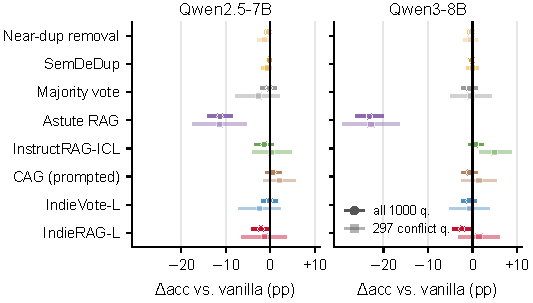
\includegraphics[width=\linewidth]{figures/web_forest.pdf}
\vspace{-5mm}
\caption{Natural web pages: paired accuracy difference to vanilla RAG with 95\% bootstrap CIs, on all 1{,}000 questions
(dark) and the 297 questions whose pages conflict (light).}
\label{fig:webforest}
\vspace{-2mm}
\end{figure}
\begin{figure}[!t]
\centering
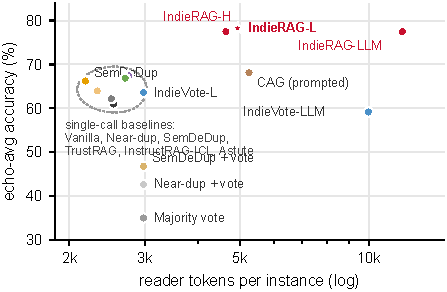
\includegraphics[width=\linewidth]{figures/cost.pdf}
\vspace{-5mm}
\caption{Echo accuracy vs.\ reader tokens per instance (Qwen2.5-7B; MADAM-RAG omitted as it ran on three conditions).}
\label{fig:cost}
\vspace{-2mm}
\end{figure}

\section{Reproducibility}\label{app:repro}
One script runs the complete pipeline (benchmark construction, all methods and statistics) as resumable jobs and caches
every LLM call. The tables in this paper are generated from the result files by a script that copies numbers
verbatim, and the figures are drawn from the raw results and per-instance predictions. Hyper-parameters: 220-word
passages; 8 copies per type; $\theta{=}0.5$; $\tau{=}1.5$; SemDeDup cosine 0.95; near-duplicate 5-gram containment 0.5;
agents use the top-3 results and at most 4 searches; bootstrap with 5{,}000 resamples clustered by question; seed 2026.

\clearpage
\end{document}
